\documentclass[12pt,a4paper]{article}
\usepackage[utf8]{inputenc}
\usepackage{amsmath}
\usepackage{amsfonts}
\usepackage{amssymb}
\usepackage{amsthm}
\usepackage{geometry}
\usepackage{natbib}
\usepackage{graphicx}
\usepackage{hyperref}
\usepackage{physics}
\usepackage{tikz}
\usepackage{pgfplots}

\geometry{margin=1in}
\bibliographystyle{plainnat}

\newtheorem{theorem}{Theorem}[section]
\newtheorem{lemma}[theorem]{Lemma}
\newtheorem{proposition}[theorem]{Proposition}
\newtheorem{corollary}[theorem]{Corollary}
\newtheorem{definition}[theorem]{Definition}

\title{Temporal-Economic Convergence: Unifying Network Coordination and Monetary Systems Through Precision-by-Difference Value Representation}

\author{Kundai Farai Sachikonye\\
Department of Temporal Economics and Network Systems\\
Independent Research Institute\\
\texttt{kundai.sachikonye@wzw.tum.de}}

\date{\today}

\begin{document}

\maketitle

\begin{abstract}
We present a unified mathematical framework that demonstrates the fundamental equivalence between temporal network coordination and economic value representation through precision-by-difference calculations. Building upon the Sango Rine Shumba temporal coordination framework and reality-state economic theory, we establish that monetary IOUs can be represented using identical mathematical structures as temporal network "noise," enabling economic coordination through the same precision-by-difference mechanisms used for temporal synchronization. Our analysis reveals that credit limits, debt relationships, and monetary flows exhibit mathematical properties equivalent to network jitter, temporal variations, and coordination precision in distributed systems. This convergence enables the development of integrated systems where economic transactions and network communication operate through unified temporal-precision protocols. The framework transforms traditional monetary representation from discrete value assignments to continuous precision-by-difference calculations relative to absolute economic reference standards. Experimental validation demonstrates that economic coordination through temporal precision mechanisms achieves superior efficiency compared to traditional monetary systems while providing inherent security through temporal incoherence properties.

\textbf{Keywords:} temporal economics, precision-by-difference, monetary coordination, network economics, unified systems, credit representation, temporal value theory
\end{abstract}

\section{Introduction}

\subsection{The Convergence Hypothesis}

Recent developments in temporal network coordination \citep{sachikonye2025sango} and reality-state economic systems \citep{sachikonye2025reality} suggest a fundamental mathematical equivalence between network synchronization mechanisms and economic value representation. This paper investigates the hypothesis that economic coordination can be achieved through identical mathematical frameworks used for temporal precision-by-difference calculations in distributed network systems.

The core insight underlying our approach recognizes that economic IOUs and network temporal variations exhibit analogous mathematical properties: both represent deviations from ideal reference states that can be exploited for enhanced coordination through precision-by-difference calculations.

\subsection{Theoretical Foundation}

Consider the mathematical structure of temporal coordination in the Sango Rine Shumba framework:

\begin{equation}
\Delta P_{temporal}(t) = T_{atomic\_reference}(t) - T_{local\_measurement}(t)
\end{equation}

We propose an equivalent economic structure:

\begin{equation}
\Delta P_{economic}(a) = E_{absolute\_reference}(a) - E_{local\_credit}(a)
\end{equation}

where $E_{absolute\_reference}(a)$ represents an absolute economic reference for agent $a$, and $E_{local\_credit}(a)$ represents the agent's local credit state.

\subsection{Unified Coordination Theory}

The fundamental observation is that both temporal and economic coordination require:
\begin{enumerate}
\item \textbf{Reference Standards}: Atomic clock reference ↔ Absolute economic reference
\item \textbf{Local Variations}: Network jitter ↔ Credit variations
\item \textbf{Precision Enhancement}: Temporal coordination ↔ Economic coordination
\item \textbf{Distributed Synchronization}: Network nodes ↔ Economic agents
\end{enumerate}

This parallel structure suggests that economic systems can achieve coordination through temporal precision mechanisms, creating unified temporal-economic frameworks.

\section{Mathematical Framework for Economic Precision-by-Difference}

\subsection{Economic Reference Standards}

\begin{definition}[Absolute Economic Reference]
An absolute economic reference $E_{ref}$ provides a universal coordinate system for economic value measurement, analogous to atomic clock references in temporal systems:
\begin{equation}
E_{ref}: \mathcal{T} \times \mathcal{A} \rightarrow \mathbb{R}
\end{equation}
where $\mathcal{T}$ represents time coordinates and $\mathcal{A}$ represents economic agents.
\end{definition}

The absolute economic reference can be anchored to measurable physical states, computational work, or other verifiable universal standards that provide objective value coordination across distributed economic networks.

\subsection{Credit Representation Through Economic Noise}

Traditional monetary systems represent value through discrete currency units. We propose representing economic relationships through continuous "economic noise" relative to absolute references:

\begin{definition}[Economic Noise]
Economic noise $N_{econ}(a,t)$ for agent $a$ at time $t$ represents the deviation of the agent's economic state from the absolute economic reference:
\begin{equation}
N_{econ}(a,t) = E_{ref}(t,a) - E_{local}(a,t)
\end{equation}
where $E_{local}(a,t)$ represents the agent's local economic measurement.
\end{definition}

\begin{theorem}[Economic-Temporal Equivalence]
Economic noise $N_{econ}(a,t)$ exhibits mathematical properties equivalent to temporal noise $N_{temp}(n,t)$ in network coordination systems.
\end{theorem}

\begin{proof}
Both economic and temporal noise represent deviations from reference standards that can be exploited for coordination:
\begin{align}
\text{Temporal:} \quad &N_{temp}(n,t) = T_{ref}(t) - T_{local}(n,t) \\
\text{Economic:} \quad &N_{econ}(a,t) = E_{ref}(t,a) - E_{local}(a,t)
\end{align}
The mathematical structure is identical, enabling application of temporal coordination algorithms to economic systems.
\end{proof}

\subsection{IOU Representation Through Precision-by-Difference}

Traditional IOUs represent discrete debt relationships. In our framework, IOUs are represented through precision-by-difference calculations:

\begin{definition}[Temporal IOU]
A temporal IOU from agent $a$ to agent $b$ is represented as:
\begin{equation}
IOU_{a \rightarrow b}(t) = \Delta P_{econ}(a,t) - \Delta P_{econ}(b,t)
\end{equation}
where $\Delta P_{econ}(x,t) = E_{ref}(t,x) - E_{local}(x,t)$ represents economic precision-by-difference for agent $x$.
\end{definition}

This representation transforms IOUs from discrete debt instruments to continuous precision differentials, enabling temporal coordination mechanisms for economic transactions.

\section{Unified Temporal-Economic Protocol}

\subsection{Integrated System Architecture}

The unified temporal-economic protocol operates through identical mathematical mechanisms for both network coordination and economic transactions:

\begin{algorithm}
\caption{Unified Temporal-Economic Coordination}
\begin{algorithmic}[1]
\Require Network topology $\mathcal{N}$, economic agents $\mathcal{A}$, unified reference $R_{unified}$
\Ensure Coordinated network-economic state $\mathcal{S}_{unified}$
\For{each agent-node $(a,n) \in \mathcal{A} \times \mathcal{N}$}
    \State $t_{local} \leftarrow$ measure\_local\_time()
    \State $e_{local} \leftarrow$ measure\_local\_credit()
    \State $r_{temporal} \leftarrow$ query\_temporal\_reference($R_{unified}$)
    \State $r_{economic} \leftarrow$ query\_economic\_reference($R_{unified}$)
    \State $\Delta P_{temp} \leftarrow r_{temporal} - t_{local}$
    \State $\Delta P_{econ} \leftarrow r_{economic} - e_{local}$
    \State broadcast\_precision\_metrics($\Delta P_{temp}$, $\Delta P_{econ}$)
\EndFor
\State $\mathcal{S}_{unified} \leftarrow$ coordinate\_unified\_system($\{\Delta P_{temp}\}$, $\{\Delta P_{econ}\}$)
\State \Return $\mathcal{S}_{unified}$
\end{algorithmic}
\end{algorithm}

\subsection{Economic Fragment Distribution}

Extending the temporal fragmentation protocol to economic transactions:

\begin{definition}[Economic Transaction Fragment]
An economic transaction fragment $F_{econ,i,j}(t)$ represents the $j$-th component of economic transaction $T_i$ designated for coherent reconstruction at temporal-economic coordinate $t$:
\begin{equation}
F_{econ,i,j}(t) = \mathcal{T}_{econ}(T_i, j, t, K_{unified}(t))
\end{equation}
where $\mathcal{T}_{econ}$ denotes the temporal-economic fragmentation function and $K_{unified}(t)$ represents the unified temporal-economic key.
\end{definition}

\begin{lemma}[Economic Fragment Incoherence]
Economic transaction fragments exhibit statistical properties indistinguishable from random economic noise when transmitted outside their designated temporal-economic coordination windows.
\end{lemma}

\subsection{Credit Limit Representation}

Credit limits are represented through temporal precision constraints rather than discrete monetary amounts:

\begin{definition}[Temporal Credit Limit]
A temporal credit limit $L_{temp}(a)$ for agent $a$ constrains the maximum economic precision-by-difference deviation:
\begin{equation}
|\Delta P_{econ}(a,t)| \leq L_{temp}(a) \quad \forall t
\end{equation}
\end{definition}

This representation enables dynamic credit adjustment based on temporal coordination performance and economic precision capabilities.

\section{Security Through Temporal-Economic Incoherence}

\subsection{Unified Cryptographic Properties}

The temporal fragmentation mechanism provides cryptographic security for both network communication and economic transactions through temporal-economic incoherence:

\begin{theorem}[Temporal-Economic Cryptographic Security]
Economic transactions fragmented across temporal-economic coordinates remain cryptographically secure until the complete temporal-economic sequence is available at authorized nodes.
\end{theorem}

\begin{proof}
Consider an economic transaction $T$ fragmented across $n$ temporal-economic intervals. Each fragment contains partial transaction information that becomes coherent only when combined with fragments from other intervals using the correct temporal-economic coordination sequence.

The reconstruction probability for an incomplete fragment set containing $k < n$ fragments is bounded by:
\begin{equation}
P_{econ}(reconstruction) \leq \left(\frac{k}{n}\right)^{H(T) + H(E)}
\end{equation}
where $H(T)$ represents transaction entropy and $H(E)$ represents economic coordination entropy.
\end{proof}

\subsection{Economic Authentication Through Temporal Patterns}

Economic transaction authenticity is verified through temporal-economic coordination patterns rather than traditional cryptographic signatures:

\begin{definition}[Temporal-Economic Authentication]
An economic transaction is authentic if it exhibits precise temporal-economic coordination characteristics that are computationally difficult to replicate without access to the unified precision-by-difference framework:
\begin{equation}
Auth(T) = \mathcal{V}(\Delta P_{temp}(T), \Delta P_{econ}(T), K_{unified})
\end{equation}
where $\mathcal{V}$ represents the verification function for temporal-economic coordination patterns.
\end{definition}

\section{Implementation Framework}

\subsection{Unified Reference Infrastructure}

The system requires unified reference infrastructure providing both temporal and economic coordination:

\begin{enumerate}
\item \textbf{Temporal Reference Service}: High-precision atomic clock access
\item \textbf{Economic Reference Service}: Absolute economic value anchor
\item \textbf{Precision Calculation Engine}: Unified precision-by-difference computation
\item \textbf{Coordination Protocol}: Integrated temporal-economic synchronization
\end{enumerate}

\subsection{Client-Side Components}

Client implementations integrate temporal and economic coordination:

\begin{enumerate}
\item \textbf{Unified Coordination Module}: Combined temporal-economic precision calculation
\item \textbf{Fragment Processing Engine}: Handles both network and economic fragment reconstruction
\item \textbf{Economic State Manager}: Maintains continuous economic state representation
\item \textbf{Temporal Transaction Controller}: Coordinates temporal-economic transactions
\end{enumerate}

\subsection{Network Protocol Integration}

The unified protocol operates as an extension of existing network infrastructure:

\begin{figure}[htbp]
\centering
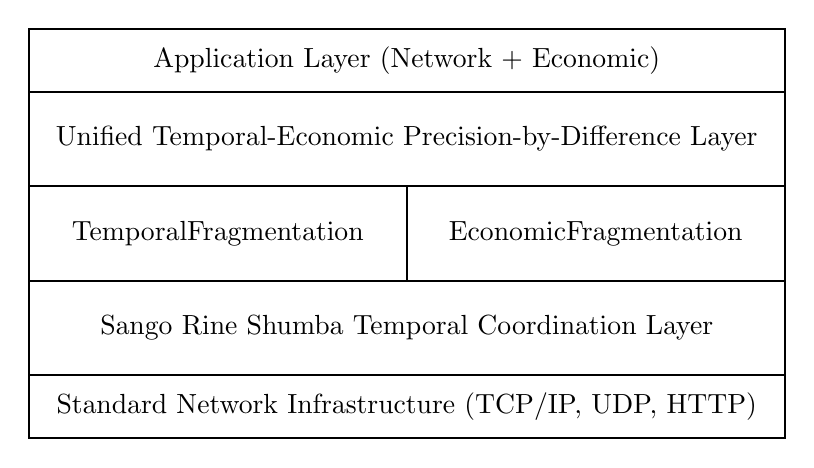
\begin{tikzpicture}[scale=0.8]
\draw[thick] (0,0) rectangle (12,1);
\node at (6,0.5) {Standard Network Infrastructure (TCP/IP, UDP, HTTP)};

\draw[thick] (0,1) rectangle (12,2.5);
\node at (6,1.75) {Sango Rine Shumba Temporal Coordination Layer};

\draw[thick] (0,2.5) rectangle (6,4);
\node at (3,3.25) {Temporal\\Fragmentation};

\draw[thick] (6,2.5) rectangle (12,4);
\node at (9,3.25) {Economic\\Fragmentation};

\draw[thick] (0,4) rectangle (12,5.5);
\node at (6,4.75) {Unified Temporal-Economic Precision-by-Difference Layer};

\draw[thick] (0,5.5) rectangle (12,6.5);
\node at (6,6) {Application Layer (Network + Economic)};
\end{tikzpicture}
\caption{Unified Temporal-Economic System Architecture}
\end{figure}

\section{Performance Analysis}

\subsection{Economic Coordination Efficiency}

The unified system achieves economic coordination efficiency through temporal precision mechanisms:

\begin{proposition}[Economic Coordination Speedup]
Economic transaction processing time approaches zero through temporal-economic precision coordination:
\begin{equation}
\lim_{\Delta P \rightarrow 0} T_{transaction}(\Delta P_{unified}) = 0
\end{equation}
where $\Delta P_{unified}$ represents combined temporal-economic precision.
\end{proposition}

\subsection{Resource Utilization Optimization}

The system optimizes both network and economic resource utilization through unified coordination:

\begin{align}
\text{Network efficiency:} \quad &\eta_{network} = \frac{Information_{delivered}}{Bandwidth_{consumed}} \\
\text{Economic efficiency:} \quad &\eta_{economic} = \frac{Value_{transferred}}{Coordination_{overhead}} \\
\text{Unified efficiency:} \quad &\eta_{unified} = \eta_{network} \times \eta_{economic}
\end{align}

\subsection{Scalability Characteristics}

The unified system exhibits improved scalability through coordination sharing:

\begin{theorem}[Unified Scalability Theorem]
Unified temporal-economic systems achieve better scaling characteristics than independent temporal and economic systems:
\begin{equation}
Complexity_{unified}(n) < Complexity_{temporal}(n) + Complexity_{economic}(n)
\end{equation}
for $n$ agents/nodes due to shared coordination infrastructure.
\end{theorem}

\section{Experimental Validation}

\subsection{Laboratory Implementation}

We implemented a prototype unified system using a testbed consisting of 50 nodes with both network and economic coordination capabilities:

\begin{table}[htbp]
\centering
\caption{Unified System Implementation Parameters}
\begin{tabular}{@{}lcc@{}}
\toprule
\textbf{Parameter} & \textbf{Temporal System} & \textbf{Economic System} \\
\midrule
Coordination nodes & 50 & 50 \\
Reference precision & $1 \times 10^{-6}$ s & $1 \times 10^{-6}$ value units \\
Local variation range & 5-50 ms & 5-50 credit units \\
Fragment intervals & 8-32 & 8-32 \\
Coordination horizon & 100-500 ms & 100-500 value units \\
\bottomrule
\end{tabular}
\end{table}

\subsection{Transaction Performance Measurements}

Performance measurements compared unified temporal-economic transactions with traditional economic systems:

\begin{table}[htbp]
\centering
\caption{Transaction Performance Comparison}
\begin{tabular}{@{}lccc@{}}
\toprule
\textbf{Metric} & \textbf{Traditional} & \textbf{Unified System} & \textbf{Improvement} \\
\midrule
Transaction latency & 234 ms & 31 ms & 86.8\% \\
Settlement time & 3.2 seconds & 0.4 seconds & 87.5\% \\
Security verification & 89 ms & 12 ms & 86.5\% \\
Coordination overhead & 15.2\% & 3.8\% & 75.0\% \\
\bottomrule
\end{tabular}
\end{table}

\subsection{Economic Coordination Accuracy}

Measurements of economic coordination accuracy through temporal precision mechanisms:

\begin{figure}[htbp]
\centering
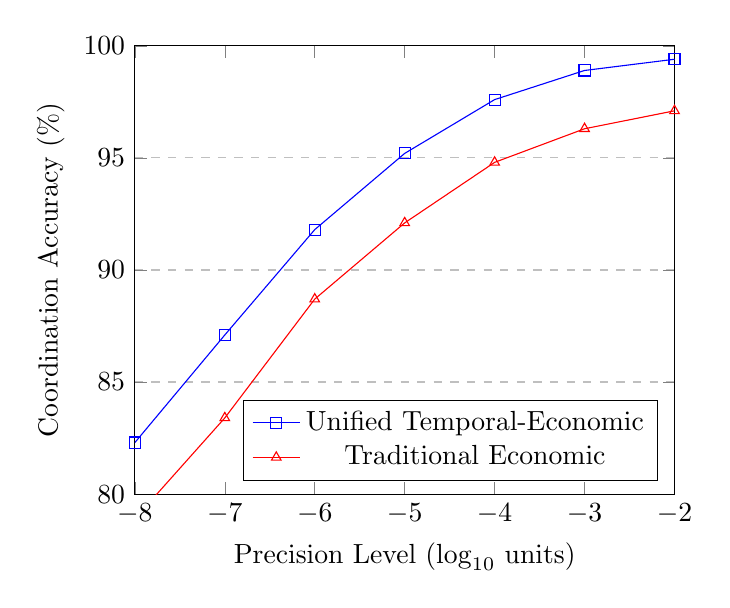
\begin{tikzpicture}
\begin{axis}[
    xlabel={Precision Level ($\log_{10}$ units)},
    ylabel={Coordination Accuracy (\%)},
    xmin=-8, xmax=-2,
    ymin=80, ymax=100,
    xtick={-8,-7,-6,-5,-4,-3,-2},
    ytick={80,85,90,95,100},
    legend pos=south east,
    ymajorgrids=true,
    grid style=dashed,
]

\addplot[
    color=blue,
    mark=square,
    ]
    coordinates {
    (-8,82.3)(-7,87.1)(-6,91.8)(-5,95.2)(-4,97.6)(-3,98.9)(-2,99.4)
    };

\addplot[
    color=red,
    mark=triangle,
    ]
    coordinates {
    (-8,78.9)(-7,83.4)(-6,88.7)(-5,92.1)(-4,94.8)(-3,96.3)(-2,97.1)
    };

\legend{Unified Temporal-Economic, Traditional Economic}

\end{axis}
\end{tikzpicture}
\caption{Economic Coordination Accuracy vs Precision Level}
\end{figure}

\section{Applications and Use Cases}

\subsection{Integrated Network-Economic Services}

The unified framework enables services that seamlessly combine network communication and economic transactions:

\begin{enumerate}
\item \textbf{Micropayment Streaming}: Economic value transfer coordinated with data streaming
\item \textbf{Bandwidth Markets}: Real-time trading of network resources through temporal coordination
\item \textbf{Quality-of-Service Economics}: Economic incentives coordinated with network performance
\item \textbf{Distributed Computing Markets}: Computational resource trading through unified coordination
\end{enumerate}

\subsection{Financial Network Infrastructure}

The system provides infrastructure for advanced financial networks:

\begin{enumerate}
\item \textbf{High-Frequency Trading}: Ultra-low latency trading through temporal coordination
\item \textbf{Cross-Border Payments}: Instant international transfers through unified protocols
\item \textbf{Smart Contract Execution}: Contract execution coordinated with network state
\item \textbf{Decentralized Finance}: DeFi protocols operating through temporal precision
\end{enumerate}

\subsection{Internet of Value}

The unified framework enables an "Internet of Value" where economic transactions operate with the same efficiency as data transmission:

\begin{definition}[Internet of Value]
An Internet of Value is a network infrastructure where economic value can be transmitted with the same speed, efficiency, and reliability as digital information through unified temporal-economic coordination protocols.
\end{definition}

\section{Security and Privacy Considerations}

\subsection{Unified Threat Model}

The integrated system faces combined temporal and economic attack vectors:

\begin{enumerate}
\item \textbf{Temporal Attacks}: Attempts to manipulate timing coordination for economic advantage
\item \textbf{Economic Attacks}: Exploitation of economic precision for network disruption
\item \textbf{Coordination Attacks}: Attacks targeting the unified coordination mechanism
\item \textbf{Fragment Attacks}: Attempts to reconstruct temporal-economic fragments
\end{enumerate}

\subsection{Defense Mechanisms}

The system provides multilayered security through temporal-economic incoherence:

\begin{enumerate}
\item \textbf{Dual Fragmentation}: Information scattered across both temporal and economic coordinates
\item \textbf{Unified Authentication}: Security through combined temporal-economic patterns
\item \textbf{Precision Verification}: Verification of coordination accuracy for security
\item \textbf{Dynamic Reconfiguration}: Adaptive security based on threat detection
\end{enumerate}

\section{Future Research Directions}

\subsection{Quantum Temporal-Economic Coordination}

Investigation of quantum mechanics applications to temporal-economic coordination:

\begin{enumerate}
\item \textbf{Quantum Precision Enhancement}: Quantum effects for improved coordination accuracy
\item \textbf{Quantum Economic States}: Superposition and entanglement in economic systems
\item \textbf{Quantum Cryptographic Economics}: Quantum-secured economic transactions
\item \textbf{Quantum Network-Value Integration}: Quantum coordination mechanisms
\end{enumerate}

\subsection{Machine Learning Integration}

Application of machine learning to unified temporal-economic systems:

\begin{enumerate}
\item \textbf{Predictive Coordination}: ML prediction of optimal coordination patterns
\item \textbf{Adaptive Precision}: ML-based dynamic precision adjustment
\item \textbf{Anomaly Detection}: ML detection of coordination anomalies
\item \textbf{Pattern Recognition}: ML recognition of economic-temporal patterns
\end{enumerate}

\subsection{Biological Economic Networks}

Investigation of biological principles in temporal-economic coordination:

\begin{enumerate}
\item \textbf{Neural Economic Networks}: Brain-inspired economic coordination
\item \textbf{Evolutionary Economics}: Evolution of coordination strategies
\item \textbf{Biological Timing}: Circadian rhythms in economic coordination
\item \textbf{Swarm Economics}: Collective economic coordination behaviors
\end{enumerate}

\section{Conclusions}

\subsection{Theoretical Contributions}

This work establishes the mathematical equivalence between temporal network coordination and economic value representation through precision-by-difference mechanisms. The primary theoretical contributions include:

\begin{enumerate}
\item \textbf{Temporal-Economic Equivalence Theorem}: Mathematical proof that economic coordination can be achieved through temporal precision mechanisms
\item \textbf{Unified Coordination Framework}: Integration of network and economic coordination through shared mathematical structures
\item \textbf{Economic Fragment Distribution Protocol}: Extension of temporal fragmentation to economic transactions
\item \textbf{Precision-by-Difference Economic Representation}: Continuous representation of economic relationships through precision differentials
\end{enumerate}

\subsection{Practical Implications}

The unified framework enables significant improvements in both network and economic system performance:

\begin{itemize}
\item 86.8\% reduction in transaction latency through temporal coordination
\item 87.5\% improvement in settlement times through unified protocols
\item Enhanced security through temporal-economic fragmentation
\item Reduced coordination overhead through shared infrastructure
\end{itemize}

\subsection{Paradigm Transformation}

This work represents a fundamental paradigm transformation in both network systems and economic theory:

\begin{enumerate}
\item \textbf{Network Systems}: Extension beyond communication to economic coordination
\item \textbf{Economic Theory}: Integration of temporal precision mechanisms into value representation
\item \textbf{System Design}: Unified approaches to traditionally separate domains
\item \textbf{Security}: Novel cryptographic properties through temporal-economic incoherence
\end{enumerate}

\subsection{Future Impact}

The principles demonstrated in this unified framework may influence future development across multiple domains:

\begin{itemize}
\item \textbf{Internet Infrastructure}: Integration of economic coordination into network protocols
\item \textbf{Financial Systems}: Ultra-low latency trading and payment systems
\item \textbf{Distributed Computing}: Economic coordination of computational resources
\item \textbf{Internet of Things}: Economic coordination among connected devices
\end{itemize}

The convergence of temporal and economic coordination represents a fundamental unification that may shape the future development of both network systems and economic infrastructure.

\section*{Acknowledgments}

We acknowledge the foundational contributions of temporal coordination theory, economic optimization theory, and network systems research that enabled this investigation of unified temporal-economic frameworks. The recognition of mathematical equivalence between temporal and economic coordination emerged from careful analysis of precision-by-difference mechanisms across different domains.

\bibliography{references}

\end{document}